\documentclass{beamer}
\usepackage{graphicx} % Required for inserting images

\usepackage[utf8]{inputenc}
\usepackage[T1]{fontenc}
\usepackage{lmodern}
\usepackage{amsmath,amssymb}
\usepackage{microtype}
\usepackage{ellipsis}
%\usepackage[ngerman]{babel}
\let\openbox\undefined
\usepackage{mathtools}
\usepackage{enumitem}
\let\openbox\undefined
\usepackage{amsthm}
\usepackage{thmtools}
\usepackage{graphicx}
\usepackage{stmaryrd}
\usepackage{tikz}
\usetikzlibrary{positioning}
\usepackage{algpseudocode}
\usepackage[absolute,overlay]{textpos}
\usepackage{url}
\usepackage[
backend=biber,
style=numeric,
]{biblatex}
\addbibresource{references.bib}
\usepackage[normalem]{ulem}
\usepackage{verbatim}
\usepackage{subcaption} % allow for subfigures

\usepackage[ruled, algosection]{algorithm2e}


\declaretheoremstyle[
  spaceabove=\parsep,
  spacebelow=0,
  headfont=\bfseries,
  notefont=\bfseries,
  notebraces={(}{)},
  bodyfont=\normalfont,
  postheadspace=.5em
]{definition}

\newtheoremstyle{plain}         % name
    {\parsep}                   % Space above
    {}                          % Space below
    {\itshape}                  % Body font
    {}                          % Indent amount
    {\bfseries}                 % Theorem head font
    {.}                         % Punctuation after theorem head
    {.5em}                      % Space after theorem head
    {\thmname{#1}\thmnumber{ #2}\thmnote{ \bfseries (#3)}}                 % Theorem head spec (can be left empty, meaning ‘normal’)

\theoremstyle{plain}

% \declaretheorem[sharenumber=algocf]{theorem}
% \declaretheorem[sharenumber=algocf]{lemma}
% \declaretheorem[sharenumber=algocf]{corollary}
\declaretheorem[sharenumber=algocf]{proposition}

% \declaretheorem[sharenumber=algocf]{definition}
% \declaretheorem[sharenumber=algocf]{example}
\declaretheorem[sharenumber=algocf]{remark}
\declaretheorem[sharenumber=algocf]{notation}

\renewcommand\qedsymbol{$\square$}

\newcommand\R{\mathbb R}
\newcommand\Z{\mathbb Z}
\newcommand\N{\mathbb N}
\newcommand\C{\mathbb C}
\newcommand{\Q}{\mathbb Q}
\newcommand{\F}{\mathbb{F}}
\newcommand{\ass}{\underline{Assume:}  }
\newcommand{\zz}{\underline{t.s.:}  }

\renewcommand{\phi}{\varphi}
\renewcommand{\epsilon}{\varepsilon}


\newcommand{\stab}{\mathrm{Stab}}
\newcommand{\conv}{\mathrm{conv}}
\newcommand{\vol}{\mathrm{vol}}
% \newcommand{\min}{\text{min}}
% \newcommand{\max}{\text{max}}
% \newcommand{\ker}{\text{ker}}
\newcommand{\im}{{\mathrm{im}}}
\newcommand{\GL}{\mathrm{GL}}
\newcommand{\Aut}{{\mathrm{Aut}}}

\newcommand{\T}{\mathcal{T}}
\renewcommand{\P}{\mathcal{P}}
\renewcommand{\L}{\mathcal{L}}

\usetheme[compress]{Berlin}
\setbeamertemplate{footline}[frame number]{}
\setbeamertemplate{navigation symbols}{}
\setbeamertemplate{footline}{}

\makeatletter
\beamer@theme@subsectionfalse%
\makeatother


\title{Computing fundamental domains of crystallographic groups}
\subtitle{With connections to topological interlocking}
\author{Lukas Schnelle}
\date{GAPDays Summer 2024}

\begin{document}

% remove dots on first slide
\frame[plain]{\titlepage}

\section{Crystallographic groups}

% Fund. Domain
% Crystallographic group
% Bieberbach
% volume of fund dom
% Dirichlet Cells
\begin{frame}
    \begin{definition}[Isometry]\label{def:isometry}
        Let $\phi:\R^n \to \R^n$ be a surjective map. 
        Then $\phi$ is called an \emph{isometry} if:
        $$
            \forall v, w \in \R^n : \pause d(v^\phi, w^\phi) = d(v,w).
        $$
        with $d(-,-)$ the Euclidean distance.\\ \pause 
        The set of all isometries of dimension $n$ is denoted as $E(n)$ and called the \emph{Euclidean group}.
    \end{definition}
    \pause
    \begin{lemma}\label{lma:isom-is-grp}
        Let $E(n)$ be the set of all isometries of a dimension $n \in \N$. \\ \pause
        Then $E(n)$ is a group with the composition of homomorphisms as the group operation. \\
        Further $E(n)$ operates on $\R^n$ by matrix vector multiplication.
    \end{lemma}
\end{frame}

\begin{frame}
    \begin{proposition}[{{\cite[Exa. 1.1, Prop. 1.6]{szczepanski2012geometry}}}]
        There is an isometry
        $$
            E(n) \cong O(n) \ltimes \R^n.
        $$
        We denote with $\phi_o$ the orthogonal part of $\phi$ and with $\phi_t$ the vector/translation part of $\phi$.
    \end{proposition}

    Then the group operation of $\phi, \psi \in E(n)$ is as follows:\pause
    $$
        (\phi_o, \phi_t) \circ (\psi_o, \psi_t) \coloneqq (\underbrace{\phi_o \circ \psi_o}_{\substack{\text{op. in }O(n)\\ \text{ i.e. comp. of maps}}}, \psi_t^{\phi_o} + \phi_t),
    $$\pause
    and the action of $E(n)$ on $\R^n$ extends to the action of $O(n) \ltimes \R^n$ on $\R^n$:\pause
    \begin{align*} \label{align:semidirect-action}
        \R^n \times ( O(n) \ltimes \R^n) \to \R^n: (v, (\phi_o, \phi_t)) \mapsto v^{(\phi_o, \phi_t)} = v^{\phi_o} + \phi_t.
    \end{align*}
\end{frame}

\begin{frame}
    \begin{definition}[System of representatives]\label{def:system-of-reps}
        Let $\lambda$ be a partition of $\R^n$ and let $\emptyset \neq V \subseteq \R^n$ be a set.\\ \pause
        Then we call $V$ a \emph{system of representatives} of the partition $\lambda$ if $V$ contains exactly one element of each class of $\lambda$.
    \end{definition} \pause

    \begin{definition}[Fundamental domain]\label{def:fund-dom}
        Let $\Gamma \leq E(n)$ be a subgroup and $F \subseteq \R^n$ a closed set.
        Then $F$ is called a \emph{fundamental domain for $\Gamma$} if:\pause
        \begin{enumerate}[label=(\roman*)]
            \item $\bigcup_{\gamma \in \Gamma} F^{\langle \gamma \rangle} = \R^n$, \pause
            \item there is a system of representatives $V \subseteq \R^n$ w.r.t.\ the partition given by the orbits of $\Gamma$ acting on $\R^n$ such that $$F^\circ \subseteq V \subseteq F.$$
        \end{enumerate}
    \end{definition}
\end{frame}

\begin{frame}
    \begin{definition}[Crystallographic group]
        Let $\Gamma \leq E(n)$ be a subgroup.
        $\Gamma$ is called a \emph{crystallographic group} if $\Gamma$ is discrete and there exists a compact fundamental domain for $\Gamma$.\\
    \end{definition}
\end{frame}

\begin{frame}
    \begin{example}
        \begin{align*}
            p4 \coloneqq \Biggl<
            &\rho \coloneqq \left( \begin{pmatrix} 0 &1 \\ -1 &0\end{pmatrix}, \begin{pmatrix} 0 \\ 0 \end{pmatrix}^T\right),\\
            &\tau_1 \coloneqq \left( \begin{pmatrix} 1 &0 \\ 0 &1\end{pmatrix}, \begin{pmatrix} 1 \\ 0 \end{pmatrix}^T\right), \\
            &\tau_2 \coloneqq \left( \begin{pmatrix} 1 &0 \\ 0 &1\end{pmatrix}, \begin{pmatrix} 0 \\ 1 \end{pmatrix}^T\right) \Biggr>
        \end{align*}
    \end{example}
\end{frame}

\begin{frame}
    \only<1>{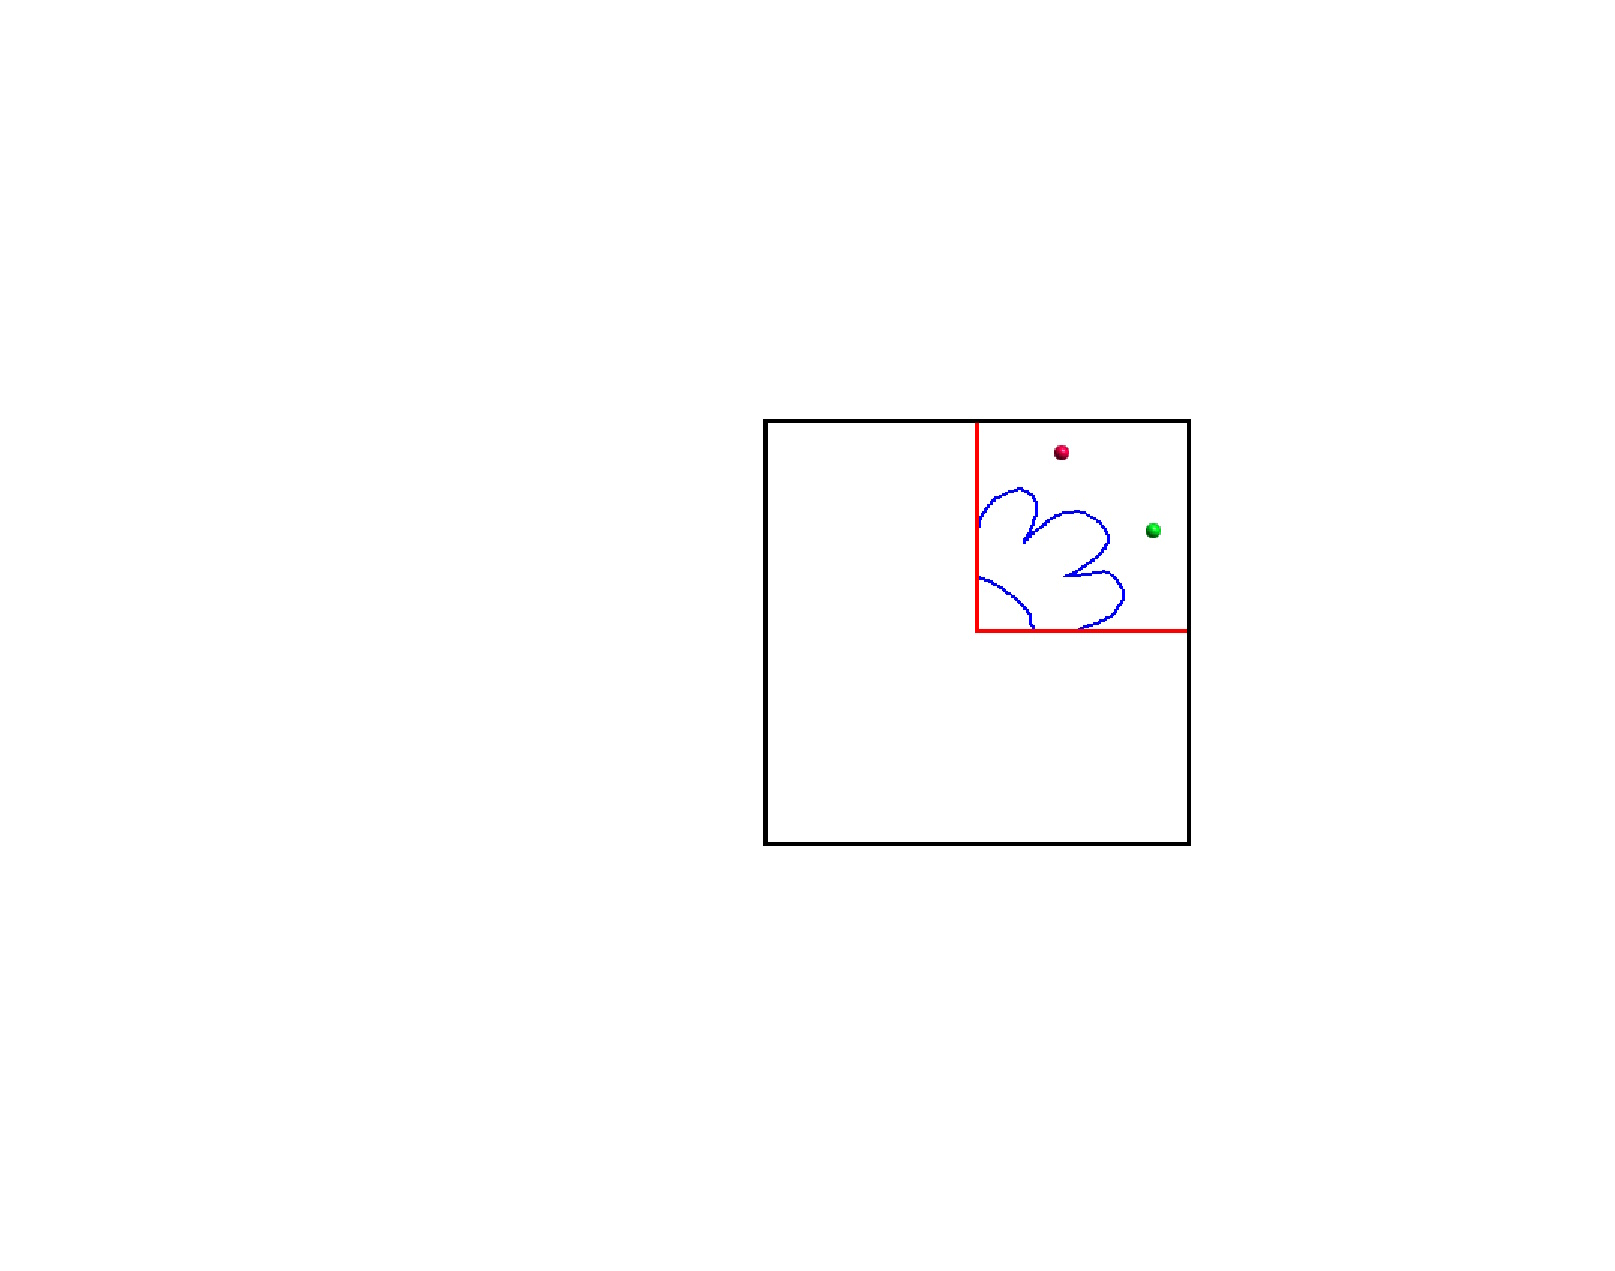
\includegraphics[width=\textwidth]{images/p4-no-rot.jpg}}
    \only<2>{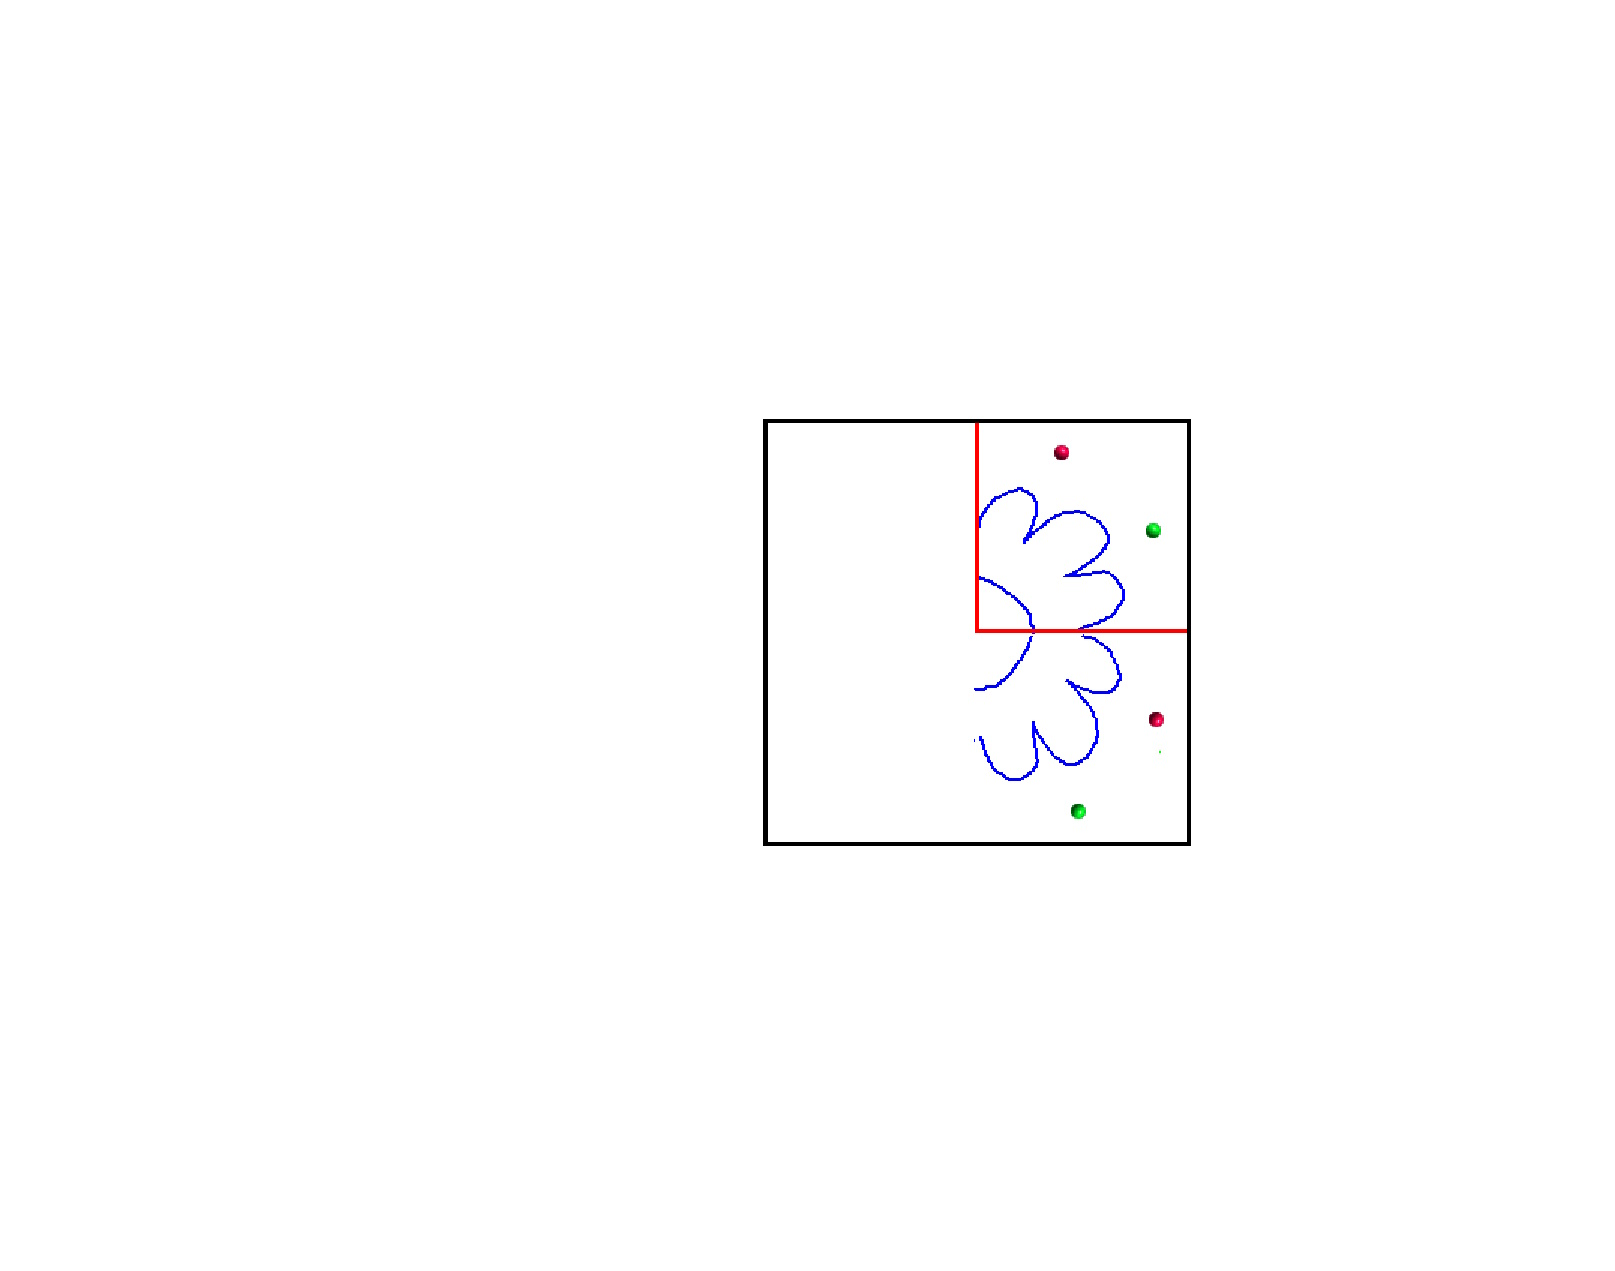
\includegraphics[width=\textwidth]{images/p4-one-rot.jpg}}
    \only<3>{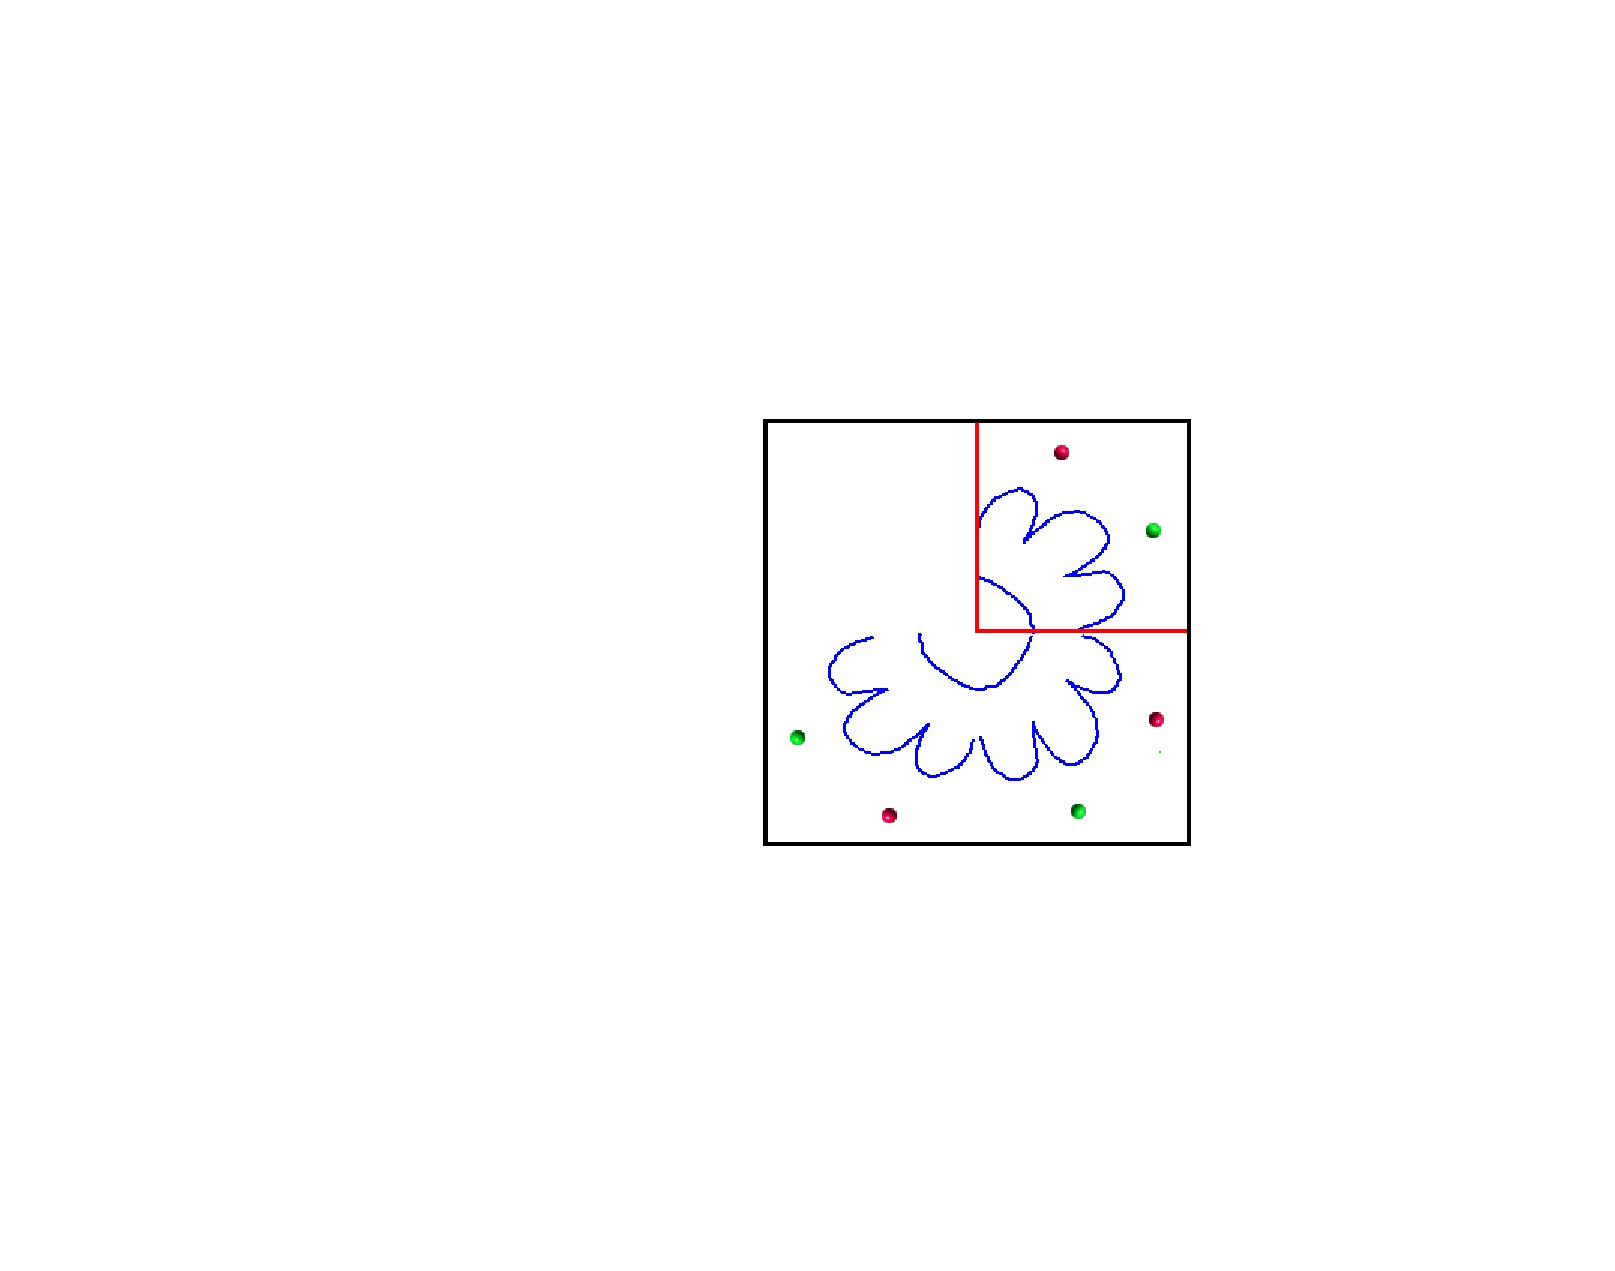
\includegraphics[width=\textwidth]{images/p4-two-rot.jpg}}
    \only<4>{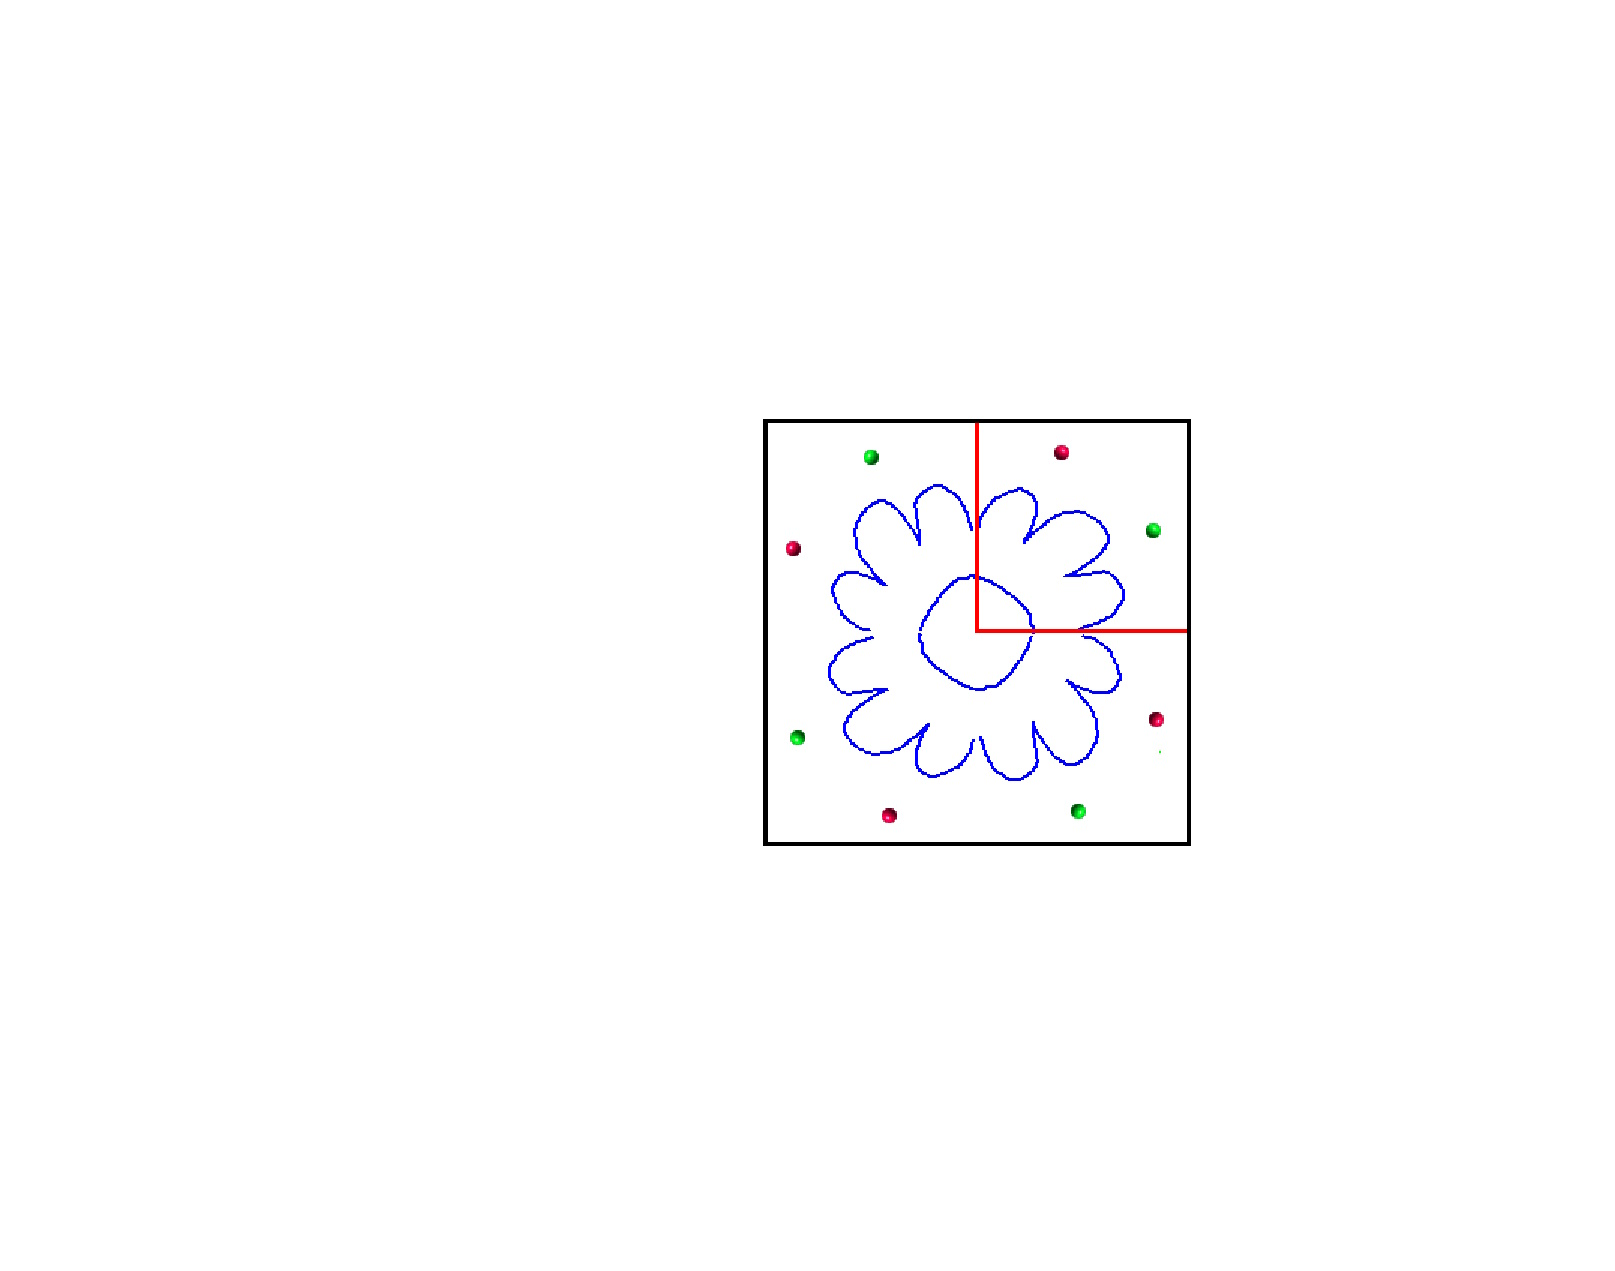
\includegraphics[width=\textwidth]{images/p4-full-rot.jpg}}
    \only<5>{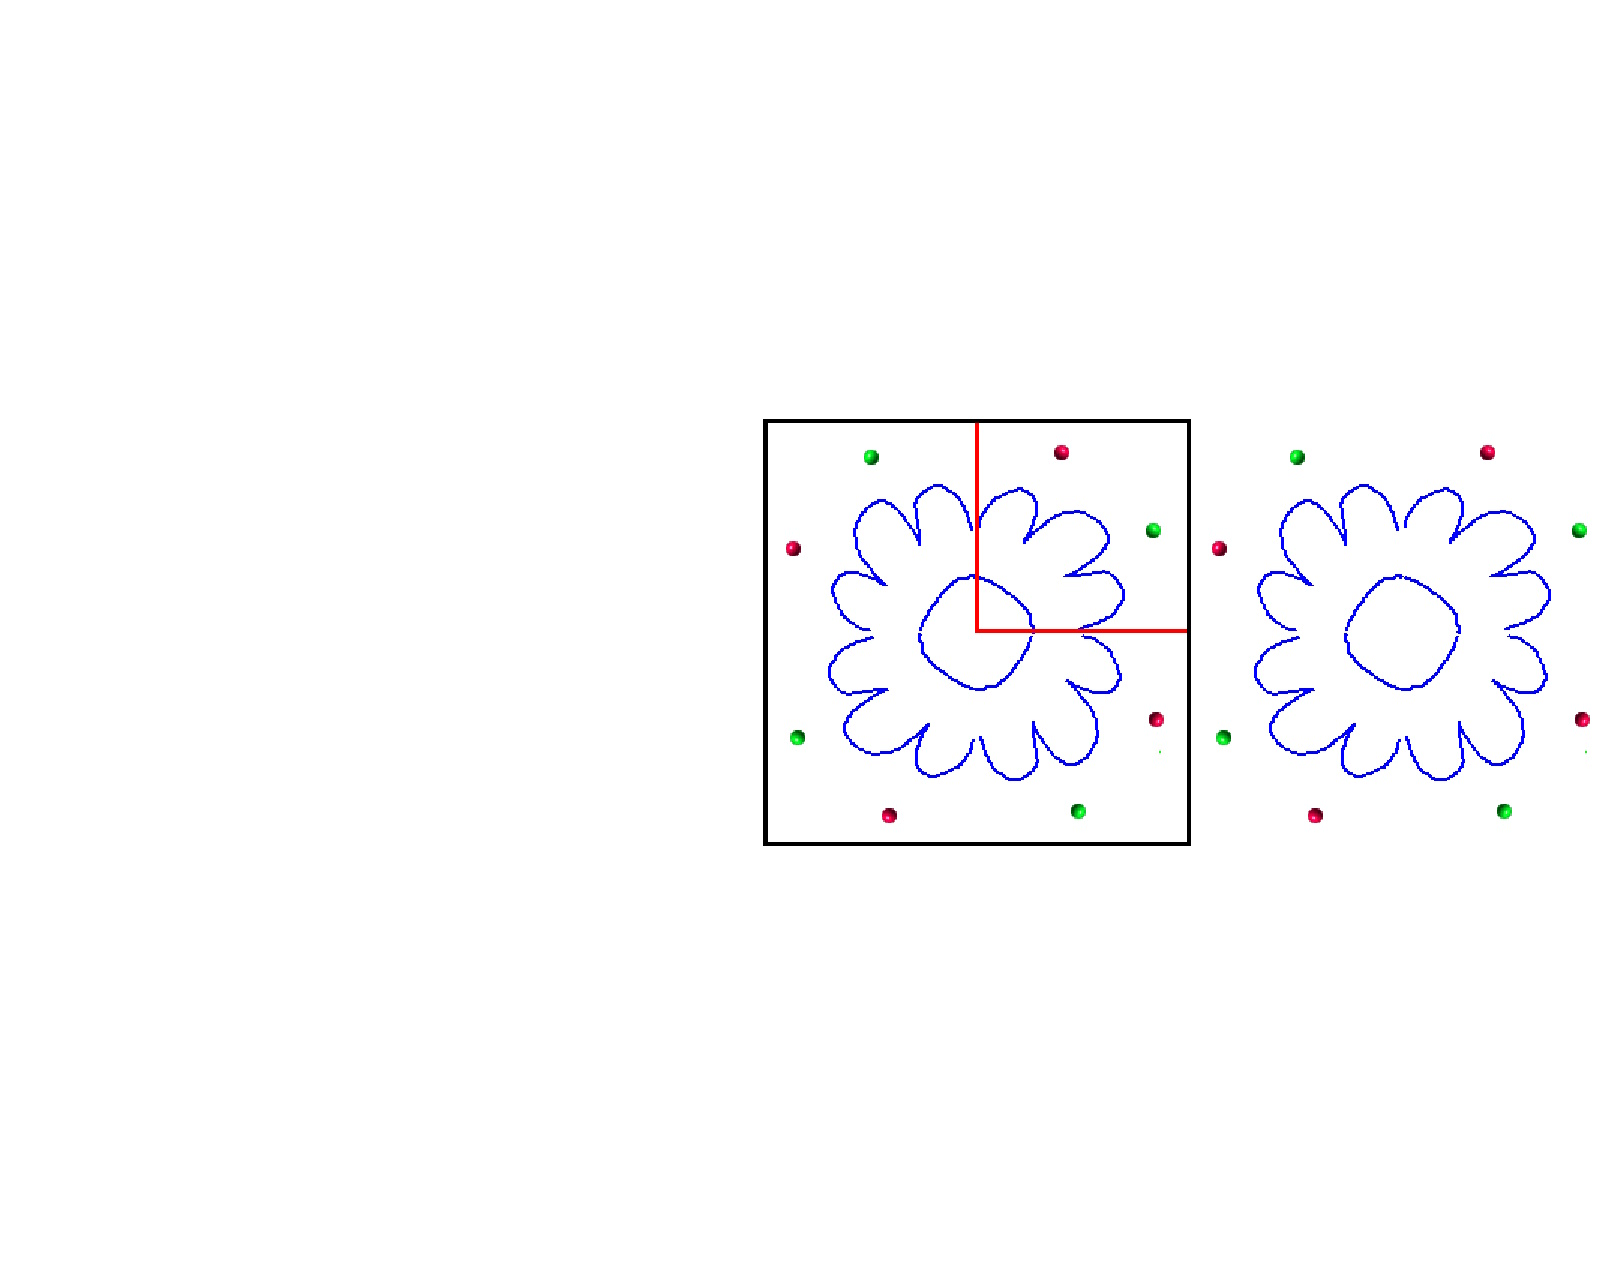
\includegraphics[width=\textwidth]{images/p4-one-trans.jpg}}
    \only<6>{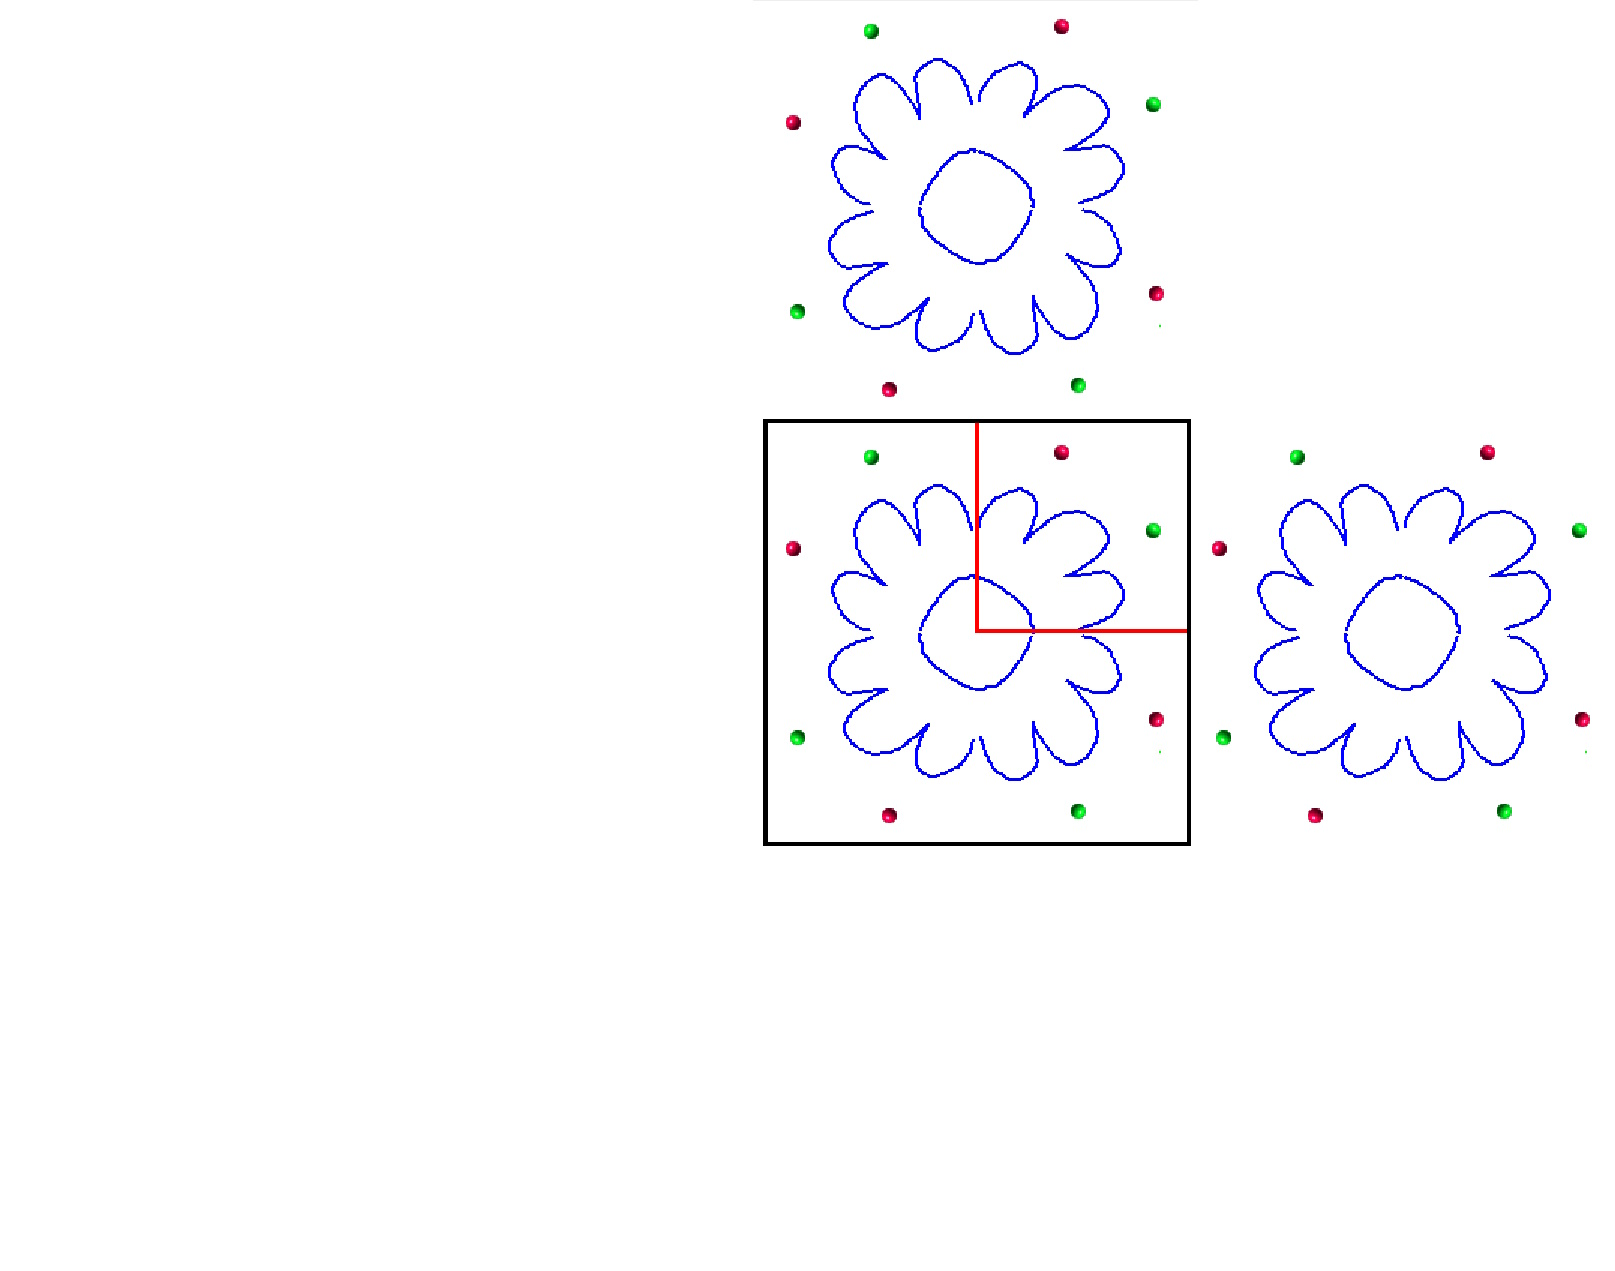
\includegraphics[width=\textwidth]{images/p4-two-trans.jpg}}
    \only<7>{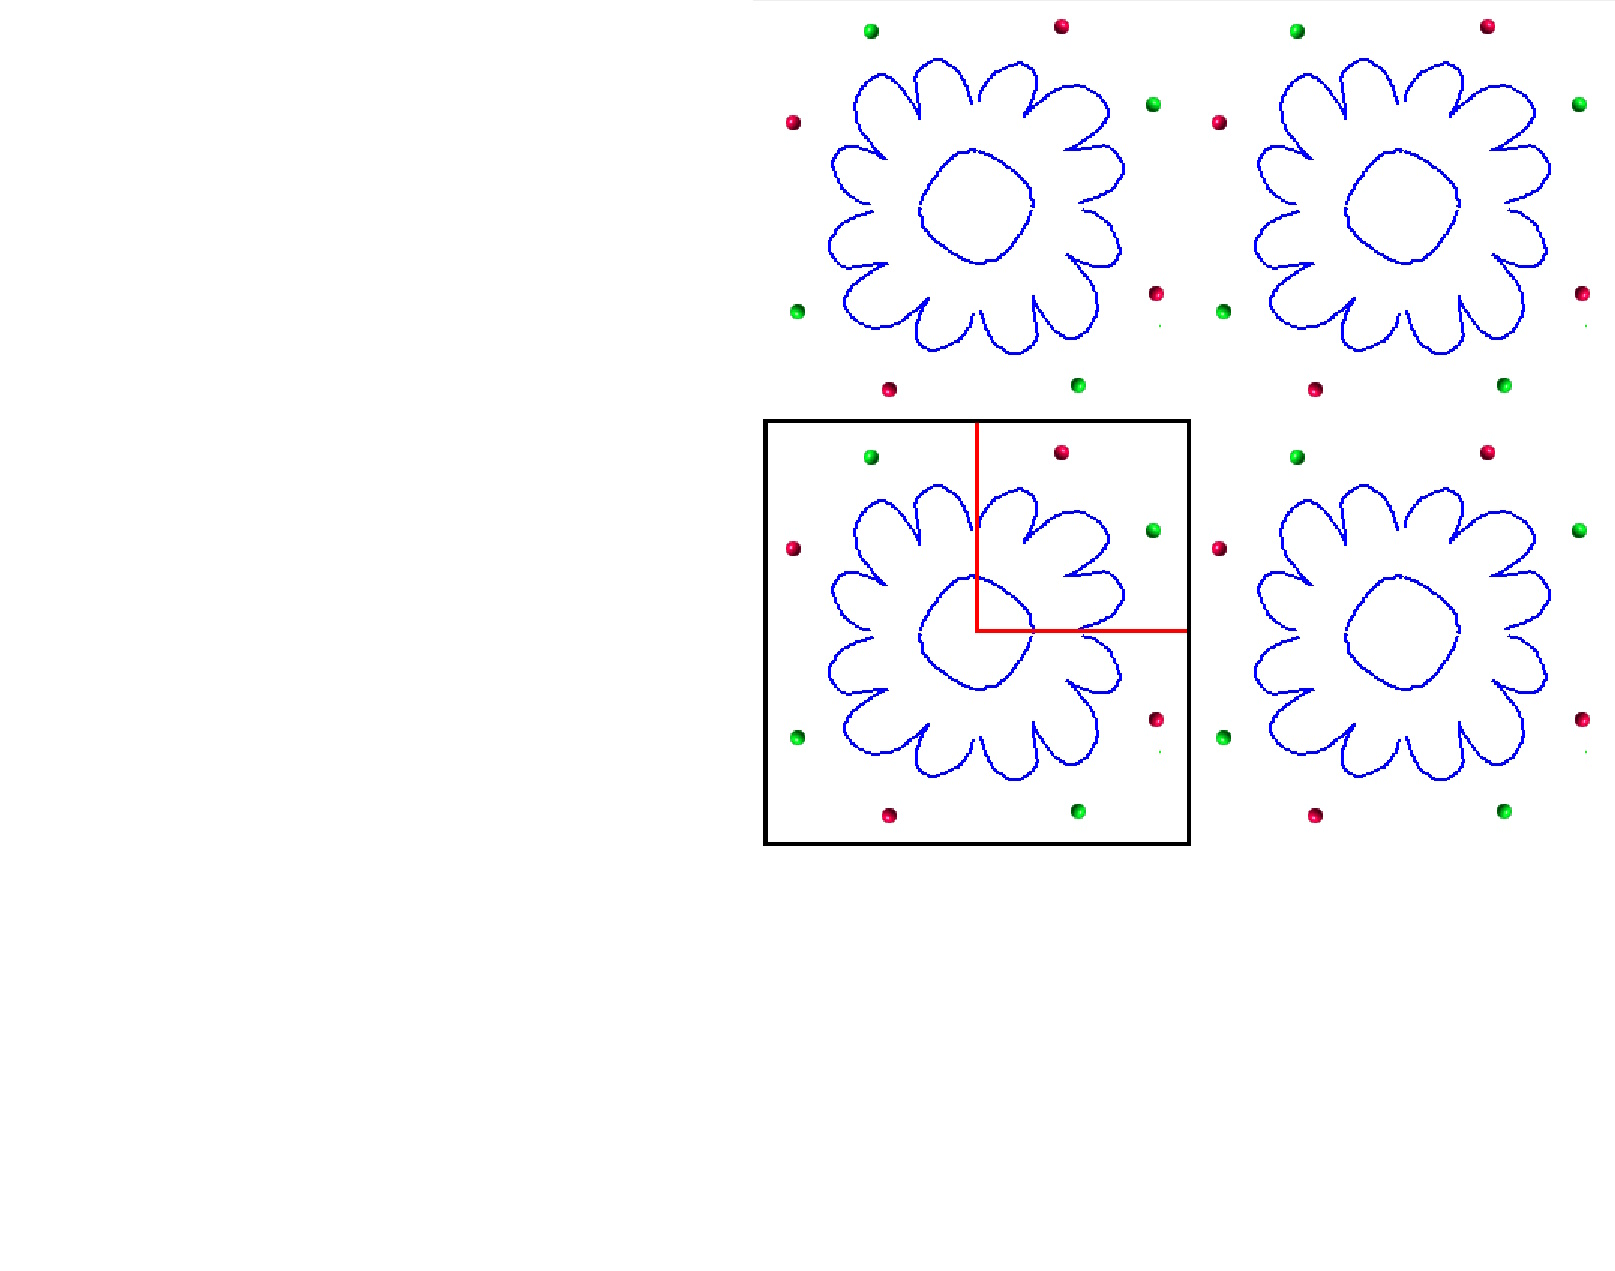
\includegraphics[width=\textwidth]{images/p4-three-trans.jpg}}
    \only<8>{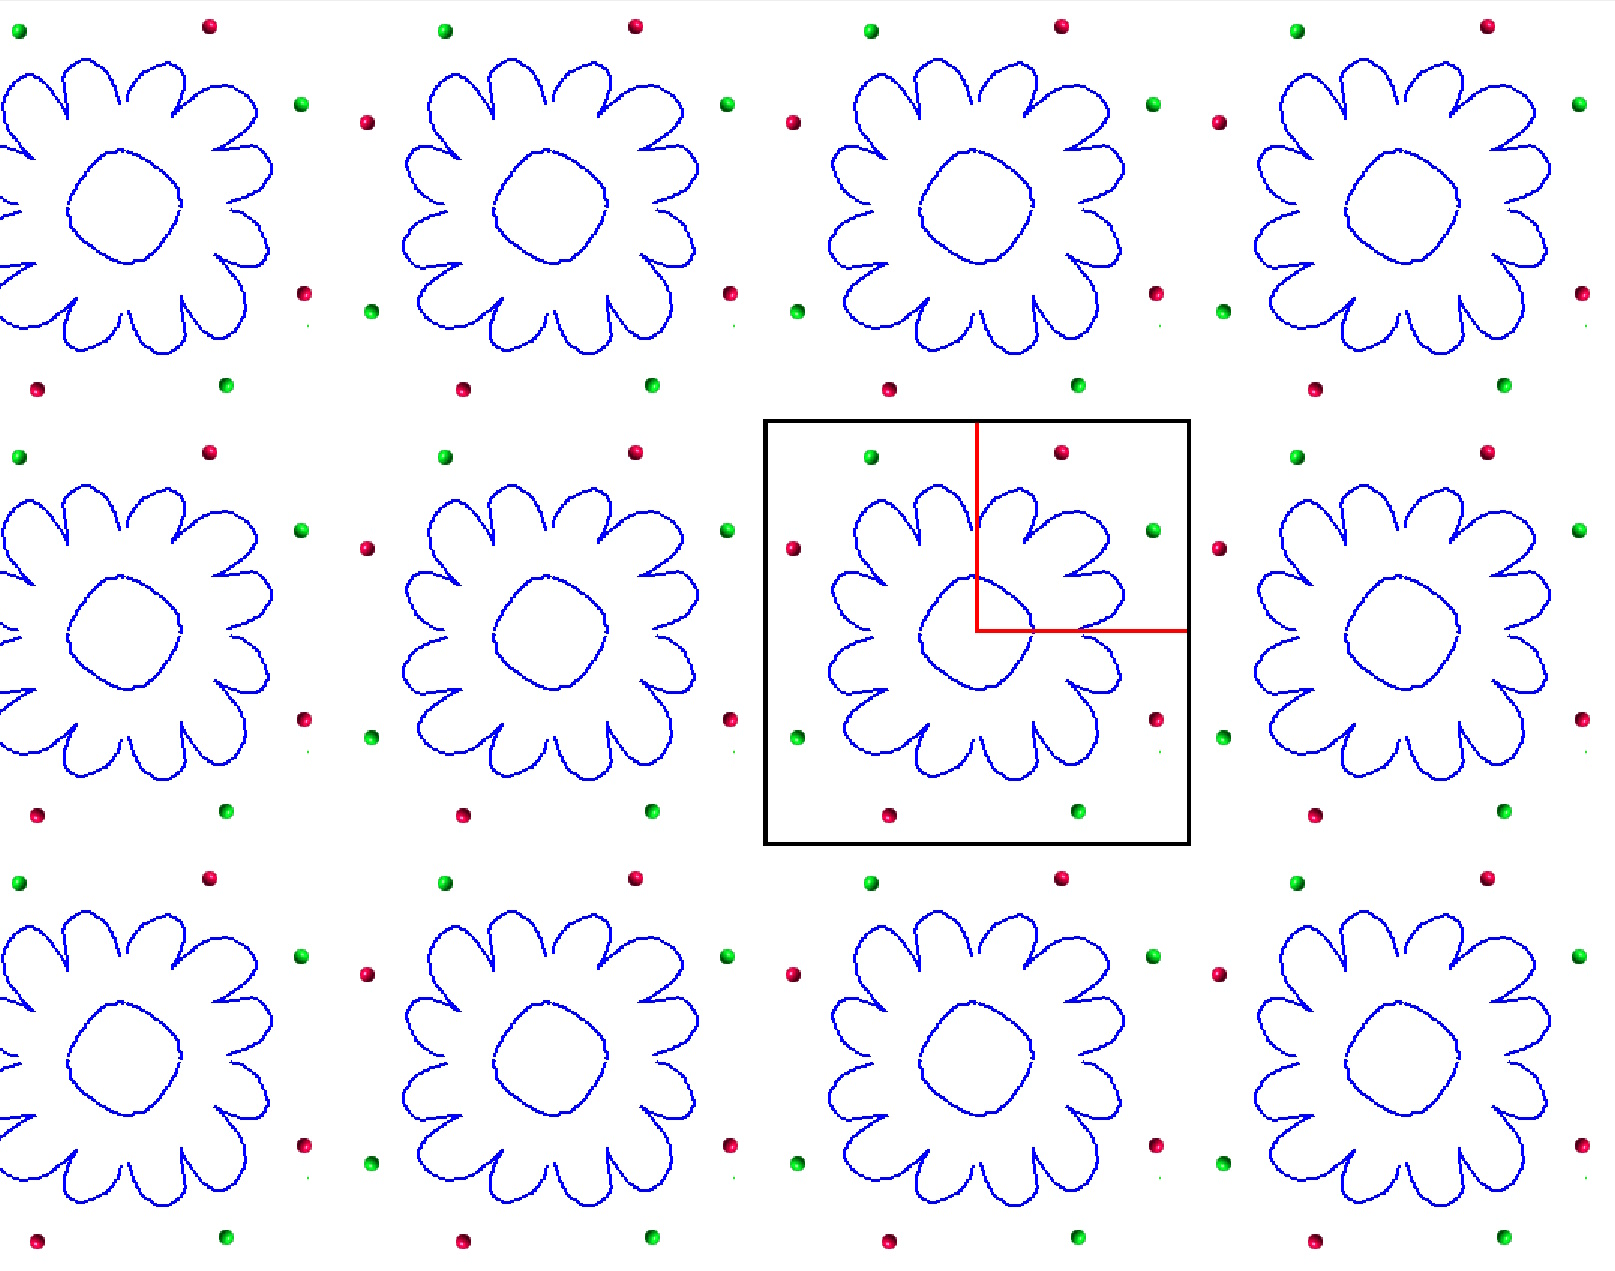
\includegraphics[width=\textwidth]{images/p4-full-trans.jpg}}
\end{frame}

\section{Dirichlet cells}
\begin{frame}
    \begin{definition}[Halfspace]\label{def:halfspace}
        Let $u, v \in \R^n$ be two points. 
        We call \pause
        $$
            H^+(u, v) \coloneqq \{ w \in \R^n \mid d(u,w) \leq d(v, w) \}
        $$
        the \emph{halfspace} which includes all points that are closer to $u$ than to $v$ (or have the same distance).
    \end{definition}\pause

    \begin{definition}Dirichlet cell [{{\cite[Def. III.1]{plesken2014}}}]
        Let $O\subseteq \R^n$ be a discrete set and $u \in O$ be a point.
        We call 
        $$
            D(u, O) = \bigcap_{w \in O, w \neq u} H^+(u, w).
        $$
        the \emph{Dirichlet cell of $u$}.
    \end{definition}
\end{frame}

\begin{frame}
    \begin{center}
        
        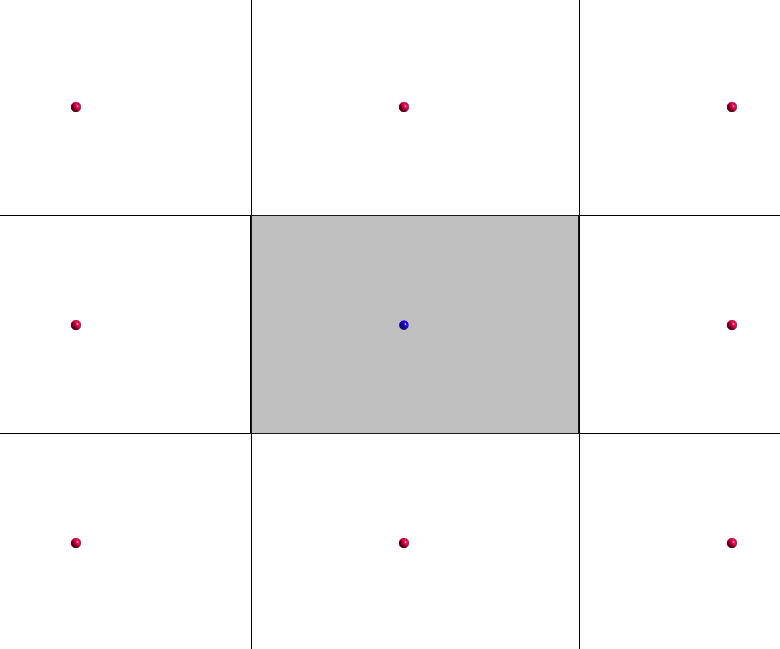
\includegraphics[width=0.9\textwidth]{images/dirichlet-example.png}
    \end{center}
\end{frame}

\begin{frame}
    \begin{definition}[Points in special/general position]\label{def:special-gen-pos}
        Let $\Gamma \leq E(n)$ be a crystallographic group and $v \in \R^n$ be a point.
        We say $v$ is in \emph{special position for $\Gamma$} if $\stab_{\Gamma}(v) \neq \{Id\}$, \pause otherwise we say $v$ is in \emph{general position for $\Gamma$}.
    \end{definition}

    \begin{theorem}[{{\cite[Thm. III.11 (ii)]{plesken1994}\label{thm:dirichlet-is-fund-dom}}}]
        Let $\Gamma \leq E(n)$ be a crystallographic group and $u \in \R^n$ a point in general position. \pause
        Then the Dirichlet cell $D(u, u^\Gamma)$ is a fundamental domain for $\Gamma$.
    \end{theorem}
    \pause
    \begin{example}
        Let $\Gamma \leq E(n)$ a crystallographic group and $u \in \R^n$ a point in general position. Then the following is a fundamental domain:
        $$
            D(u, u^\Gamma) = \bigcap_{w^\gamma, \gamma \in \Gamma \setminus \{ Id \}} H^+(u, w).
        $$
    \end{example}
\end{frame}

\section{Computational aspects}
\begin{frame}
    \begin{definition}[Volume]
        Let $B\subset \R^n$ be a closed subset. 
        We define the \emph{volume} of $B$ as the Lebesgue measure of $B$, so $\vol(B) \coloneqq \lambda(B)$ in the notation of \cite{forster2012analysis3}. 
    \end{definition} \pause

    \begin{theorem}[{{\cite[§3, Thm. 2]{forster2012analysis3}\label{thm:vol-invar-under-isom}}}]
        Let $B \subset \R^3$ a closed subset, $\phi \in E(3)$. \\ \pause
        Then $vol(B^\phi) = vol(B)$.
    \end{theorem}
    \pause
    It can be shown that all fundamental domains of crystallographic groups have the same volume.
\end{frame}

\begin{frame}
    \begin{remark}
        For every crystallographic group $\Gamma$ there is a certain subgroup called the translation subgroup that is denoted by 
        $$
            \T(\Gamma) \leq \Gamma.
        $$
    \end{remark}
\end{frame}

\begin{frame}
    \begin{theorem}
        Let $\Gamma \leq E(n)$ be a crystallographic group with fundamental domain $F$ and $u \in \R^n$ a point in general position. Then we choose a generating set for $\Gamma$ and $I, K$ finite index sets, such that
        $$
            \Gamma = \langle \rho_i, \tau_k \mid i \in I, k \in K \rangle,
        $$\pause
        with $\tau_k \in \T(\Gamma)$ for all $k \in K$ and $\{ (\tau_k)_t \mid k \in K \}$ are a basis for the lattice induced by $\T(\Gamma)$. Furthermore, let $\rho_i \in \Gamma$  for $i \in I$ be chosen such that 
        $$
            \Gamma = \bigcup_{i \in I} \rho_i \T(\Gamma).
        $$\pause
        Then there is an $A \in \N$ such that the Dirichlet cell $D(u, u^\Gamma)$ is the intersection of halfspaces $H^+(u,w)$ for words $w$ of length at most $A+1$.
    \end{theorem}
\end{frame}

\begin{frame}
    \begin{algorithm}[H]
        \caption{Dirichlet Cell}\label{alg:dirichletcell}
        \LinesNumberedHidden
        \SetAlgoLined
        \KwData{a crystallographic group $\Gamma = \langle \rho_i, \tau_k \mid i \in I, k \in K \rangle \leq E(n)$ such that $\Gamma = \cup_{i \in I} \rho_i \T(\Gamma)$, a point $u$ in general position w.r.t. $\Gamma$ and the maximal $length$ of words in $gens$ to check}
        \KwResult{$triangularComplex$, a triangular complex that is a fundamental domain. }
        % initialization\;
        $wordsOfLenghtL$ $\leftarrow$ all words in the generators $gens$ of length at most $length$\,
        
        % \tcp{generate orbit of $u$ under action of $wordsOfLenghtL$}
        % elementsInOrbit := []\;
        \For{ $\gamma$ in wordsOfLenghtL}{
            Add(elementsInOrbit, $u^\gamma$)\;
        }
    
        $halfspaces \leftarrow$ halfspaces $H_{u,v}$ for all $v \in elementsInOrbit$\;
    
        $fundDom \leftarrow$ triangular complex given by intersection of $halfspaces$ (done with polymake(ing))\;
    
        return $fundDom$\;
    \end{algorithm}
\end{frame}

\begin{frame}
    \begin{center}
        \textbf{Time for some examples}
    \end{center}
\end{frame}

\section{Outlook}
\begin{frame}
    \begin{exampleblock}{Current state}
        Previously presented algorithm is already programmed in as part of my masters thesis.
    \end{exampleblock}\pause
    \begin{block}{Next steps}
        \begin{itemize}[label={-}]
            \item Implement the algorithm in SimplicialSurfaces Package \pause
            \item Improve algorithm by automatically running until expected volume is reached \pause
            \item Check if $h$-vector conversion can be done more efficiently \pause
            \item Consider numerical effects \pause
        \end{itemize}
    \end{block}
    
\end{frame}

\begin{frame}
    \begin{exampleblock}{Motivation}
        Goal is to deform fundamental domains in such a way, that they continue to be fundamental domains but also fulfill the \emph{topological interlocking property}.
    \end{exampleblock}\pause
    \begin{definition}{Topologically interlocking}
        A block $B \subseteq \R^3$ is called topologically interlocking, if there is an assembly of it, such that by fixing a subset of the assembly there is no subset of the remaining blocks that can be moved without intersecting any blocks.
    \end{definition}
\end{frame}

\begin{frame}
    \textbf{\Large Thank you for your attention}\\ 
    \bigskip
    References:\\
    \printbibliography
\end{frame}

\end{document}
